\section{Inference}
\subsection{Alpha-BP}
{ \setbeamercolor{background canvas}{bg=hl_bg}
  \setbeamercolor{normal text}{fg=hl_fg}
  \setbeamercolor{frametitle}{fg=hl_fg}
  \begin{frame}
    \usebeamercolor[fg]{normal text}
    \begin{center}
      {
        \begin{tikzpicture}
          \tikzstyle{cnode} = [thick, draw=white, ellipse, inner sep = 2pt,  align=center]
          \tikzstyle{fnode} = [thick, draw=white, ellipse, inner sep = 10pt,  align=center]
          \tikzstyle{rnode} = [thick, rectangle, inner sep = 1.5pt,  align=left]
          \node[rnode] (inf) at (-2, 0) {\large Inference};
          \node[rnode, below = 0.6cm of inf.west, anchor=west, draw=green] (abp) {$\bullet$ \textbf{$\alpha$-BP}};
          \node[rnode, below = 1.2cm of inf.west, anchor=west] (renn) {$\bullet$ RENN};
          \node[cnode, fit=(abp)(inf)(renn)] (infn) {};
          
          \node[rnode, right = 3 of inf] (lern) {\large Learning};
          \node[rnode, below = 0.4 of lern.west, anchor=west] (genmm) {$\bullet$ GenMM};
          \node[rnode, below = 0.8 of lern.west, anchor=west] (genhmm) {{$\bullet$} GenHMM};
          \node[rnode, below = 1.2 of lern.west, anchor=west] (lfree) {{$\bullet$} EOTGM};
          \node[cnode, fit=(lern)(genmm)(genhmm)(lfree)] (learn) {};

          \node[fnode, fit=(infn)(lern)] (box) {};

          
          \node[below right = 0.5 and -0.5 of infn] {{Probabilistic} Graphical Model};
          \draw[->,line width=0.2mm] (infn) to[out=15, in=165] (learn);
          \draw[->,line width=0.2mm] (learn) to[out=195, in=-15] (infn);
        \end{tikzpicture}
      }
    \end{center}
    
  \end{frame}
}

\begin{frame}{Alternative Veiw of BP: $\alpha$-BP}
  Input:
  \begin{columns}
    \column{0.45\textwidth}
    \begin{itemize}[label=$\bullet$]
    \item A pairwise Markov random field: $p(\bm{x}) \propto \prod_{{s\in \Vv}} \phi_s(x_s) \prod_{(s,t) \in \Ee} \phi_{st}(x_s, x_t)$
    \item A trial distribution: $q(\bm{x}) \propto \prod_{{s\in \Vv}} \tilde{\phi}_s(x_s) \prod_{(s,t) \in \Ee} \tilde{\phi}_{st}(x_s, x_t)$ with factorization $\tilde{\phi}_{s,t}(x_s, x_t) := m_{st}(x_t) m_{ts}(x_s)$
    \item A metric: $\alpha$-Divergence 
    \end{itemize}
    
    \column{0.55\textwidth}
    \begin{tikzpicture}
      \begin{scope}[scale=0.8, every node/.append style={transform shape}]
        \tikzstyle{enode} = [thick, draw=black, circle, inner sep = 4pt, minimum size = 0.7cm, align=center]
        \tikzstyle{nnode} = [thick, rectangle, rounded corners = 0pt, minimum size = 0.5cm,draw,inner sep = 2pt]
        \tikzstyle{cnode} = [thick, cloud, draw,cloud puffs=10, cloud puff arc=120, aspect=2, inner ysep=4pt]
        \node[cnode] (pajk) at (3, 1.5) {$\Nn(t)\backslash s$};
        \node[cnode] (paik) at (-3, 1.5) {$\Nn(s)\backslash t$};
        \node[nnode] (tk) at (0, 1.5) {};
        \node[] at ($(tk) + (0, 0.5)$) {$\phi_{st}(x_s, x_t)$};
        \node[enode] (xi) at (-1.5 ,0) {};
        \node[] at ($(xi) + (0.75,0)$) {$x_s$};
        \node[nnode] (fi) at (-1.5 , -1.5) {};
        \node[] at ($(fi) + (0.95,0)$) {$\phi_s(x_s)$};
        \node[enode] (xj) at (1.5 ,0) {};
        \node[] at ($(xj) + (0.75,0)$) {$x_t$};
        \node[nnode] (fj) at (1.5 , -1.5) {};
        \node[] at ($(fj) + (0.95,0)$) {$\phi_t(x_t)$};
        % connections
        \draw[-] (xi) to (fi);
        \draw[-] (xi) to (tk);
        \draw[-] (xi) to (paik);
        \draw[-] (xj) to (fj);
        \draw[-] (xj) to (tk);
        \draw[-] (xj) to (pajk);
      \end{scope}
    \end{tikzpicture}
    \centering{$\Gg_F:=(\Vv \cup \Ff, \Ee_F)$}
  \end{columns}
  \vskip 1cm

  \let\thefootnote\relax\footnotetext{\tiny
    \vskip -0.2cm
    Definition of $\alpha$-divergence $\Dd_{\alpha}(p \| q ) = \frac{\sum_{\bm{x}} \alpha p(\bm{x}) + (1-\alpha) q (\bm{x}) - p(\bm{x})^{\alpha} q(\bm{x})^{1-\alpha}}{\alpha(1-\alpha)}$\\
      Approximate local minimization:
  \begin{itemize}[label=$\bullet$]
  \item Direct minimization: $ \!\!\!\uargmin{\tilde{\phi}_{ts}^{\mathrm{new}}(x_t, x_s)}\!\!\!\! \Dd_{\alpha_{ts}}\!\!\left(  p^{\backslash (t,s)}\!(\bm{x})\phi_{ts}(x_t, x_s)\|q^{\backslash (t,s)}\!(\bm{x})\tilde{\phi}_{ts}^{\mathrm{new}}(x_t, x_s)\right)$
  \item Local minimization: $\!\!\!\uargmin{\tilde{\phi}_{ts}^{\mathrm{new}}(x_t, x_s)}\!\!\!\!  \Dd_{\alpha_{ts}}\!\!\left( q^{\backslash (t,s)}\!(\bm{x}){\phi}_{ts}(x_t, x_s) \|q^{\backslash (t,s)}\!(\bm{x})\tilde{\phi}_{ts}^{\mathrm{new}}(x_t, x_s) \right)$, say you are updating $\tilde{\phi}_{ts}^{\mathrm{new}}(x_t, x_s) = m_{ts}^{\mathrm{new}}(x_s) m_{st}(x_t)$
  \end{itemize}
  }
\end{frame}

\begin{frame}
  \begin{columns}
    \column{0.5\textwidth}
    Updating message via $\alpha$-BP:
    \column{0.5\textwidth}

    \begin{tikzpicture}
      \begin{scope}[scale=0.7, shift={(-3,-4.5)}, every node/.append style={transform shape}, local bounding box=mmrfToy]
        \tikzstyle{enode} = [thick, draw=black, circle, inner sep = 4pt, align=center]
        \tikzstyle{nnode} = [thick, rectangle, rounded corners = 0pt, minimum size = 0.5cm,draw,inner sep = 2pt]
        
        \node[enode, label=above:{t}] (t) at (0 ,0) {};
        \node[nnode, label=above:{$\phi_{st}$}, right=of t] (phiSt) {};
        \node[enode, label=above:{s}, right=of phiSt] (s) {};
        \node[nnode, label=above:{w}, above left= 0.5 and 1 of t] (w) {};
        \node[label=above:{...}, left= of t] (w1) {};
        \node[nnode, below left= 0.5 and 1 of t] (w2) {};

        \draw[->] (w) -- node[midway,above=1em]{$m_{wt}$} (t);
        \draw[->] (w2) to (t);
        \draw[->] (t) to (phiSt);
        \draw[->] (phiSt) to node[midway,above=1em]{$m_{st}$} (s);

      \end{scope}
    \end{tikzpicture}
  \end{columns}
  \vskip -0.3cm
  \begin{align*}
    \underbrace{{m}^{\mathrm{new}}_{ts}(x_s)}_{\text{new msg. to s}} \propto
    \underbrace{m_{ts}(x_s)^{1-\alpha_{ts}}}_{\text{old msg. to s}} \bigg[\sum_{x_t} \phi_{ts}(x_t, x_s)^{\alpha_{ts}} \underbrace{{m}_{st}(x_t)^{1-\alpha_{ts}}}_{\text{old msg. to t}} \underbrace{{\phi}_t(x_t) \prod_{w\in \Nn(t)\backslash s}m_{wt}(x_t)}_{\text{msg. from variable node $t$ to factor $\phi_{st}$}} \bigg].
  \end{align*}
  
  \centering
  \begin{tikzpicture}
    \tikzstyle{enode} = [thick, draw, circle, inner sep = 2pt, align=center]
    \tikzstyle{nnode} = [thick, rectangle, rounded corners = 4pt, minimum size = 0.8cm,draw,inner sep = 2pt]
    \tikzstyle{cnode} = [thick, cloud, draw, cloud puffs=10, cloud puff arc=120, aspect=2, inner ysep=4pt]

    \begin{scope}
      
      \node[nnode] (Problem) at (-4, 0) {Problem};
      \node[nnode, right= of Problem] (pGraph) 
      {MRF
      };
      \node[enode, right=of pGraph] (alpha) {$\alpha$-BP};
      \node[nnode, right=of alpha] (surrogate) {
        \begin{tabular}{c}
          Surrogate \\
          Distribution
        \end{tabular}};
      \node[nnode, below=of surrogate] (sol) {Solution};

      \node[nnode, below=of Problem, opacity=0.5] (ext) {\begin{tabular}{c}Exterior \\ Estimator\end{tabular}};
      \node[nnode, right=of ext, opacity=0.5] (mmrf) {\begin{tabular}{c}Modified\\MRF\end{tabular}};
      

      \draw[green,->] (Problem) to (pGraph);
      \draw[green,->] (pGraph) to (alpha);
      \draw[green,->] (alpha) to (surrogate);
      \draw[green,->] (surrogate) to (sol);
      \draw[dashed, ->, opacity=0.5] (Problem) to (ext);
      \draw[dashed, ->, opacity=0.5] (ext) to (mmrf);
      \draw[dashed, ->, opacity=0.5] (mmrf) to (alpha);

    \end{scope}
    \begin{scope}[scale=0.7, shift={(-3.5,-4.1)}, every node/.append style={transform shape}, local bounding box=mmrfToy, opacity=0.5]
      \tikzstyle{enode} = [thick, draw=black, circle, inner sep = 4pt, minimum size = 0.7cm, align=center]
      \tikzstyle{nnode} = [thick, rectangle, rounded corners = 0pt, minimum size = 0.5cm,draw,inner sep = 2pt]
      \tikzstyle{cnode} = [thick, cloud, draw,cloud puffs=10, cloud puff arc=120, aspect=2, inner ysep=4pt]

      \node[cnode] (paik) at (-2, 0) {$\Nn(s)$};
      \node[enode] (xi) at (0 ,0) {};
      \node[] at ($(xi) + (0,0.6)$) {$x_s$};

      \node[nnode] (fi) at (0 , -1.5) {};
      \node[] at ($(fi) + (0.95, 0)$) {$\phi_s(x_s)$};

      \node[nnode] (pi) at (2, 0) {};
      \node[] at ($(pi) + (0, 0.6)$) {$\hat{p}_s(x_s)$};
      % connections
      \draw[-] (xi) to (fi);
      \draw[-] (xi) to (pi);
      \draw[-] (xi) to (paik);
    \end{scope}
    \node[nnode, fit=(mmrf)(ext)(mmrfToy), inner sep=8pt, dashed,draw=black!40] {};
  \end{tikzpicture}
\end{frame}

\begin{frame}
  \begin{columns}
    \column{0.5\textwidth}
    Updating message via $\alpha$-BP:
    \column{0.5\textwidth}

    \begin{tikzpicture}
      \begin{scope}[scale=0.7, shift={(-3,-4.5)}, every node/.append style={transform shape}, local bounding box=mmrfToy]
        \tikzstyle{enode} = [thick, draw=black, circle, inner sep = 4pt, align=center]
        \tikzstyle{nnode} = [thick, rectangle, rounded corners = 0pt, minimum size = 0.5cm,draw,inner sep = 2pt]
        
        \node[enode, label=above:{t}] (t) at (0 ,0) {};
        \node[nnode, label=above:{$\phi_{st}$}, right=of t] (phiSt) {};
        \node[enode, label=above:{s}, right=of phiSt] (s) {};
        \node[nnode, label=above:{w}, above left= 0.5 and 1 of t] (w) {};
        \node[label=above:{...}, left= of t] (w1) {};
        \node[nnode, below left= 0.5 and 1 of t] (w2) {};

        \draw[->] (w) -- node[midway,above=1em]{$m_{wt}$} (t);
        \draw[->] (w2) to (t);
        \draw[->] (t) to (phiSt);
        \draw[->] (phiSt) to node[midway,above=1em]{$m_{st}$} (s);

      \end{scope}
    \end{tikzpicture}
  \end{columns}
  \vskip -0.3cm
  \begin{align*}
    \underbrace{{m}^{\mathrm{new}}_{ts}(x_s)}_{\text{new msg. to s}} \propto
    \underbrace{m_{ts}(x_s)^{1-\alpha_{ts}}}_{\text{old msg. to s}} \bigg[\sum_{x_t} \phi_{ts}(x_t, x_s)^{\alpha_{ts}} \underbrace{{m}_{st}(x_t)^{1-\alpha_{ts}}}_{\text{old msg. to t}} \underbrace{{\phi}_t(x_t) \prod_{w\in \Nn(t)\backslash s}m_{wt}(x_t)}_{\text{msg. from variable node $t$ to factor $\phi_{st}$}} \bigg].
  \end{align*}
  \centering
  \begin{tikzpicture}
    \tikzstyle{enode} = [thick, draw, circle, inner sep = 2pt, align=center]
    \tikzstyle{nnode} = [thick, rectangle, rounded corners = 4pt, minimum size = 0.8cm,draw,inner sep = 2pt]
    \tikzstyle{cnode} = [thick, cloud, draw, cloud puffs=10, cloud puff arc=120, aspect=2, inner ysep=4pt]

    \begin{scope}
      
      \node[nnode] (Problem) at (-4, 0) {Problem};
      \node[nnode, right= of Problem, opacity=0.5] (pGraph) 
      {MRF
      };
      \node[enode, right=of pGraph] (alpha) {$\alpha$-BP};
      \node[nnode, right=of alpha] (surrogate) {
        \begin{tabular}{c}
          Surrogate \\
          Distribution
        \end{tabular}};
      \node[nnode, below=of surrogate] (sol) {Solution};

      \node[nnode, below= of Problem] (ext) {\begin{tabular}{c}Exterior \\ Estimator\end{tabular}};
      \node[nnode, right=of ext] (mmrf) {\begin{tabular}{c}Modified\\MRF\end{tabular}};
      

      \draw[dashed,->,opacity=0.5] (Problem) to (pGraph);
      \draw[dashed,->,opacity=0.5] (pGraph) to (alpha);
      \draw[green,->] (alpha) to (surrogate);
      \draw[green,->] (surrogate) to (sol);
      \draw[green, ->] (Problem) to (ext);
      \draw[green, ->] (ext) to (mmrf);
      \draw[green, ->] (mmrf) to (alpha);

    \end{scope}
    \begin{scope}[scale=0.7, shift={(-3.5,-4.1)}, every node/.append style={transform shape}, local bounding box=mmrfToy]
      \tikzstyle{enode} = [thick, draw=black, circle, inner sep = 4pt, minimum size = 0.7cm, align=center]
      \tikzstyle{nnode} = [thick, rectangle, rounded corners = 0pt, minimum size = 0.5cm,draw,inner sep = 2pt]
      \tikzstyle{cnode} = [thick, cloud, draw,cloud puffs=10, cloud puff arc=120, aspect=2, inner ysep=4pt]

      \node[cnode] (paik) at (-2, 0) {$\Nn(s)$};
      \node[enode] (xi) at (0 ,0) {};
      \node[] at ($(xi) + (0,0.6)$) {$x_s$};

      \node[nnode] (fi) at (0 , -1.5) {};
      \node[] at ($(fi) + (0.95, 0)$) {$\phi_s(x_s)$};

      \node[nnode] (pi) at (2, 0) {};
      \node[] at ($(pi) + (0, 0.6)$) {$\hat{p}_s(x_s)$};
      % connections
      \draw[-] (xi) to (fi);
      \draw[-] (xi) to (pi);
      \draw[-] (xi) to (paik);
    \end{scope}
    \node[nnode, fit=(mmrf)(ext)(mmrfToy), inner sep=8pt, dashed,draw=black!40] {};
  \end{tikzpicture}
  
\end{frame}

\begin{frame}{Insights of $\alpha$-BP}
  \begin{columns}
    \column{0.5\textwidth}
    \begin{block}{\small Connection to standard BP}
      \begin{itemize}[label=$\bullet$]
      \item $\alpha \rightarrow 0$ 
      \item $\alpha$-divergence reduces to KL-divergence
      \item Update rule of $\alpha$-BP reduces to ${m}^{\text{new}}_{ts}(x_s) \propto \sum_{x_t} \phi_{st}(x_s, x_t) {\phi}_t(x_t) \prod_{w\in \Nn(t)\backslash s}m_{wt}(x_t)$, which is standard BP update rule
        
      \end{itemize}
    \end{block}
    \column{0.45\textwidth}
    \begin{block}{\small Convergence}
      For an arbitrary pairwise Markov random field over binary variables,
      if the largest singular value of matrix $\bm{M}(\bm{\alpha}, \bm{\theta})$ is less than one,
      $\alpha$-BP converges to a fixed point. The associated fixed point is unique.
      \vfill
      {\tiny See Corollary 3.1 for relaxed condition where singular value computation is avoided.}
    \end{block}
  \end{columns}
  \vskip 0.5cm
  \begin{block}{\small What does that mean}
    \begin{itemize}[label=$\bullet$]
    \item You can safely use $\alpha$-BP as an alternative to (loopy) BP
    \item You can use matrix $\bm{M}$ to check if you are guaranteed to get stable solution from $\alpha$-BP
    \end{itemize}
  \end{block}
  \let\thefootnote\relax\footnotetext{\tiny
    \vskip -0.2cm
    \begin{columns}
      \column{0.5\textwidth}
      For binary, symmetric log-potentials 
      \begin{align*}
        \phi_{st}(x_s, x_t) &= \exp\left\{ \theta_{st}(x_s, x_t)\right\}, \nonumber \\
        \phi_{s}(x_s) &= \exp\left\{ \theta_{s}(x_s) \right\}.
      \end{align*}
      \column{0.5\textwidth}
      Matrix $\bm{M}(\bm{\alpha}, \bm{\theta})$, size $\abs{\vec{\Ee}} \times \abs{\vec{\Ee}}$, indexed by directed edges $(t\rightarrow s)$, as
      \begin{align*}
        M_{(t\rightarrow s), (u \rightarrow v)} =
        \begin{cases}
          \abs{ 1 - \alpha_{ts}}, &\quad u=t, v=s, \\
          \abs{ 1 - \alpha_{ts}} \tanh \abs{\alpha_{ts} \theta_{ts}}, & \quad u = s, v =t, \\
          \tanh\abs{\alpha_{ts} \theta_{ts}}, & \quad u \in \Nn(t)\backslash s, v = t, \\
          0, & \quad \mathrm{otherwise}.
        \end{cases}
      \end{align*}
    \end{columns}
  }
\end{frame}
\begin{frame}{Some Numerical Results}
  
  \graphicspath{{../source/chapter3/}}
  \begin{columns}
    \column{0.5\textwidth}
    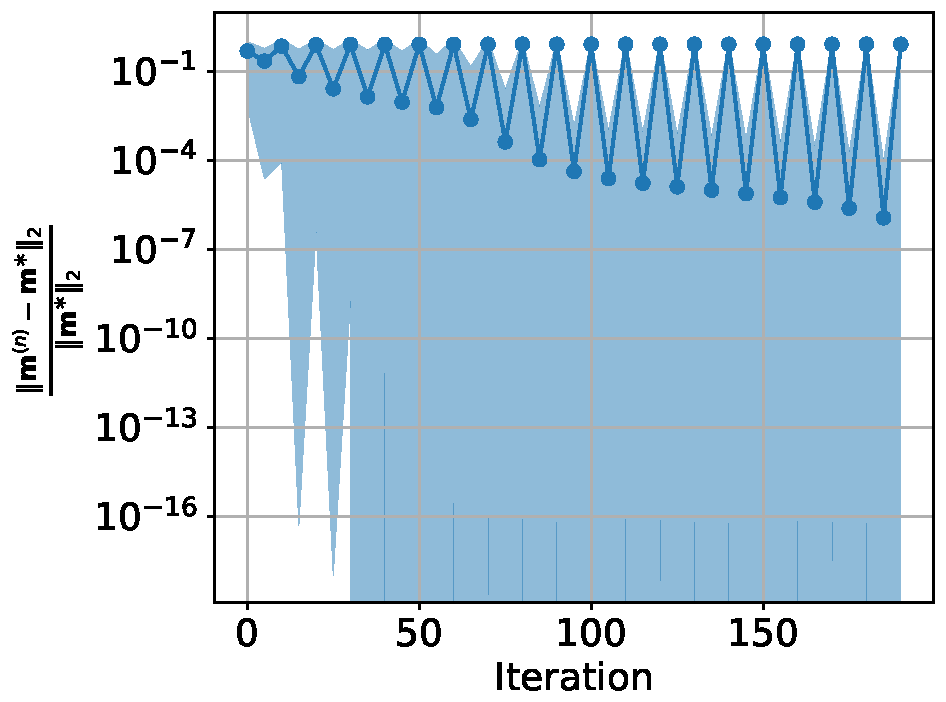
\includegraphics[width=0.8\columnwidth]{figures/converge/converge_erp0_4_alpha_1_stn_0_5_vs_filter_false_crop.pdf}
    \column{0.5\textwidth}
    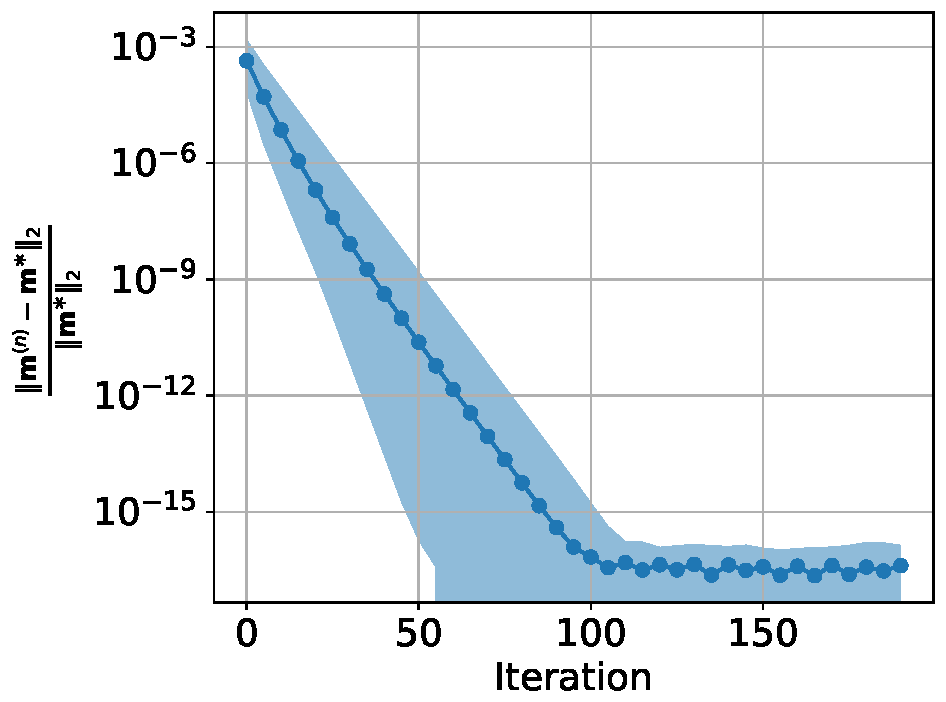
\includegraphics[width=0.8\columnwidth]{figures/converge/converge_erp0_2_alpha_0_5_stn_0_1_vs_filter_true-crop.pdf}
  \end{columns}
  \centering
  {Numerical illustration of convergence, with normalized error ${\normd{\bm{m}^{(n)}-\bm{m}^{\ast}}}/{\normd{\bm{m}^{\ast}}}$ versus the number of iterations. Blue region: range of the normalized error of $100$ graph realizations. Curve: mean error of the $100$ realized graphs. }

\end{frame}

\begin{frame}{Some Numerical Results}
  \graphicspath{{../source/chapter3/}}
  % \begin{columns}
  %   \column{0.5\textwidth}
  %   \begin{center}
  %     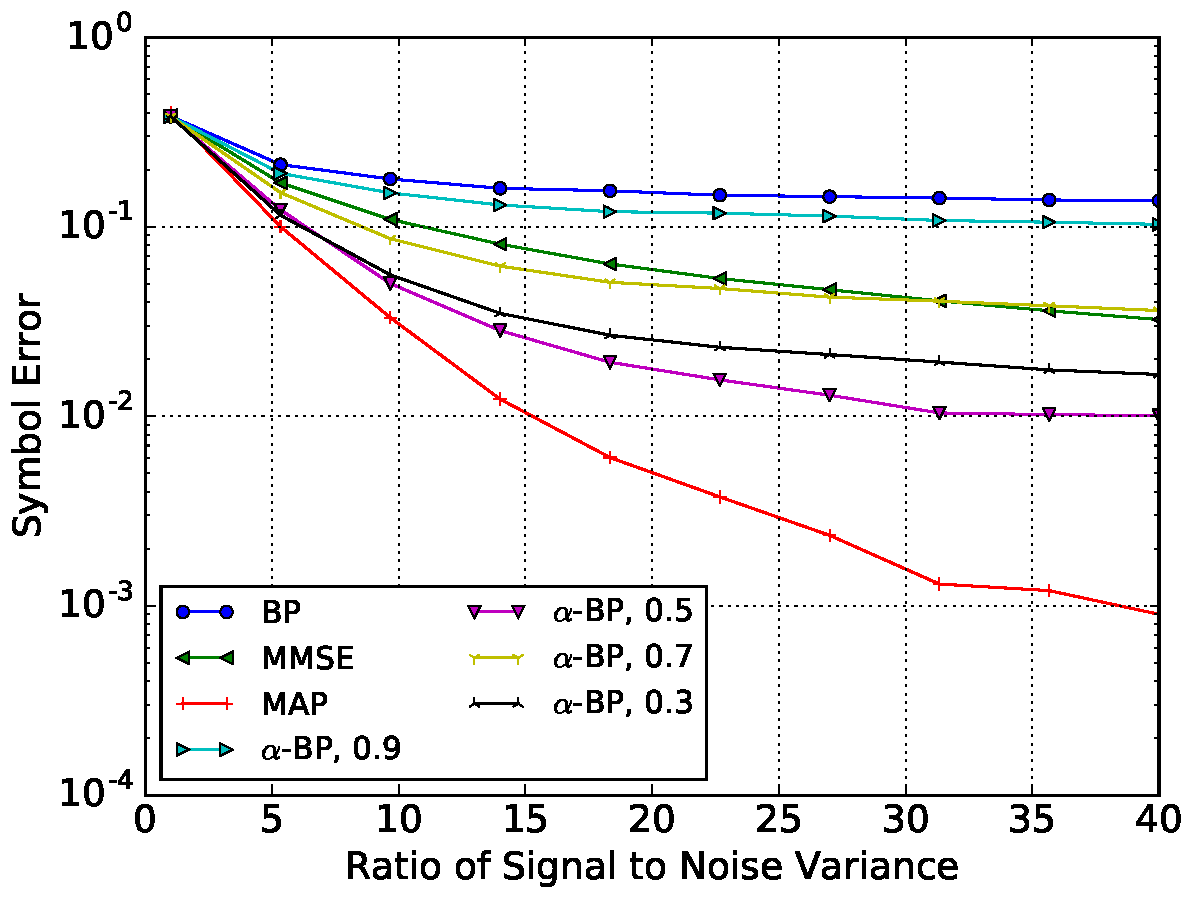
\includegraphics[width=0.8\columnwidth]{figures/alpha_compare_crop.pdf}
  %   \end{center}
  %   \column{0.5\textwidth}
  %   \centering
  %   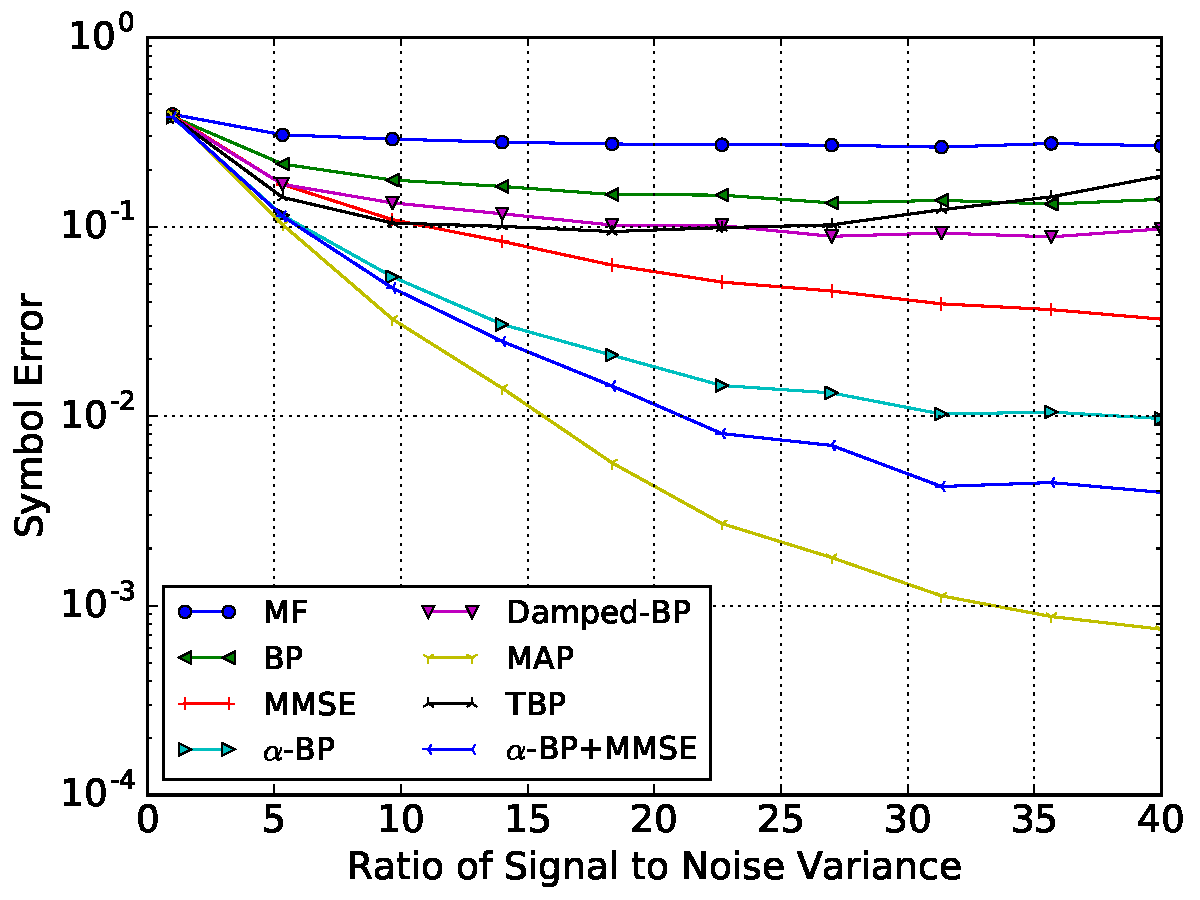
\includegraphics[width=0.8\columnwidth]{figures/tbp/mf_tbp_compare.pdf}
  % \end{columns}
  \centering
  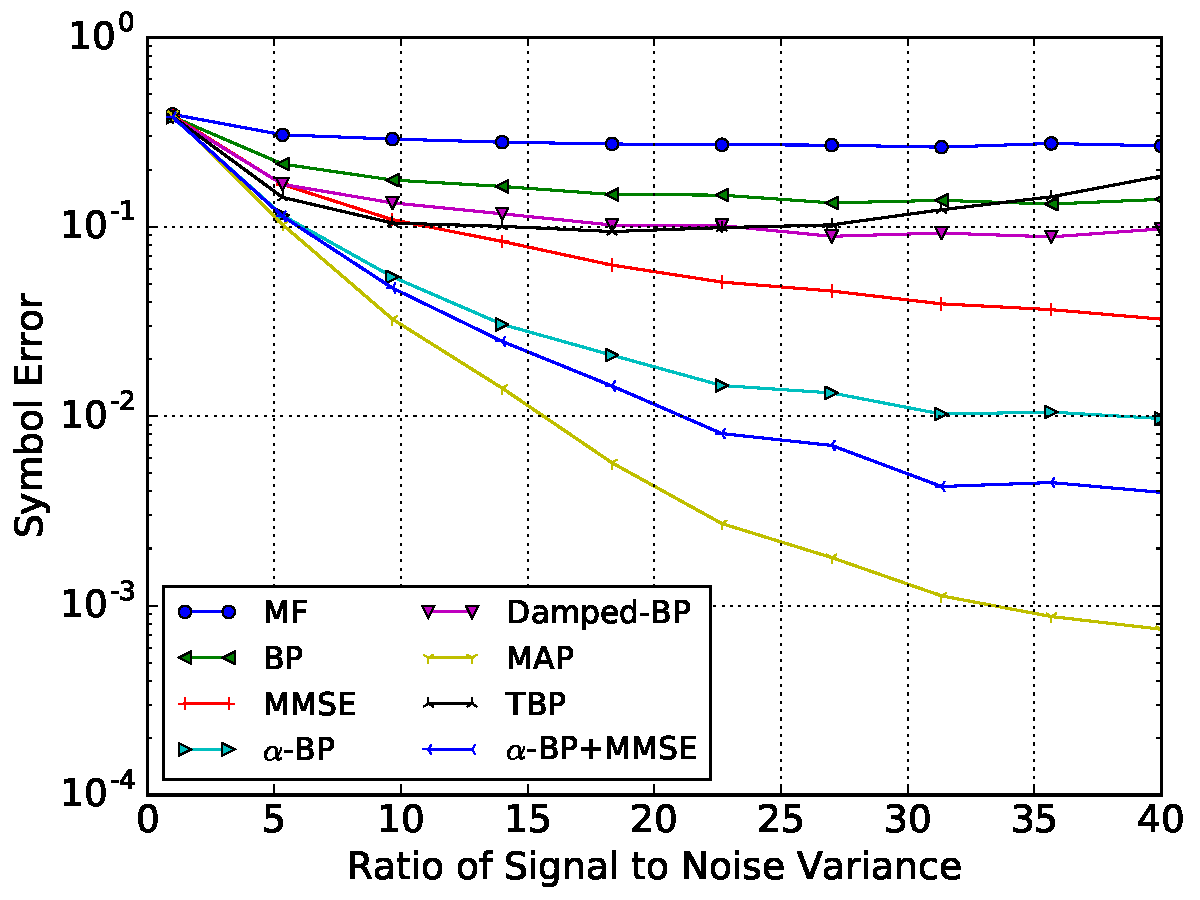
\includegraphics[width=0.5\textwidth]{figures/tbp/mf_tbp_compare.pdf}

  \centering
  {Numerical results of $\alpha$-BP: symbol error of MIMO detection.}

\end{frame}


% \subsection{GraphNet}

% \begin{frame}{Learn the message update rule by NN}
%   An end-to-end learning process: Factor graph $\rightarrow$ converted graph representation $\rightarrow$ GNN $\rightarrow$ Output
%   \begin{figure}
%     \centerline{\includegraphics[scale=0.3]{images/gnn.png}}
%   \end{figure}
%   \begin{itemize}[label=$\bullet$]
%   \item sum-product update rule (in BP) $\rightarrow$ NN, to learn
%   \item pseudo probability (belief aggregation) $\rightarrow$ NN, to learn
%   \item end-to-end learning that requires true marginal probability, which BP, GPB and mean field do no require
%   \end{itemize}
%   \let\thefootnote\relax\footnotetext{\tiny For related methods, see:\\
%   Heess et al, Learning to Pass Expectation Propagation Messages\\
%   Yoon, et al, 2019, Inference in Probabilistic Graphical Models by Graph Neural Networks\\
%   Gilmer, et al, 2017, Neural message passing for quantum chemistry.\\
%   Battaglia, et al, 2018, Relational inductive biases, deep learning, and graph networks
% }
% \end{frame}

% \subsection{AutoEncoder}

% \begin{frame}
%   {Variational Auto-encoder}
%   \onslide<1->{
%   \begin{itemize}[label=$\bullet$]
%   \item Simplification on structures \\
%     \begin{tikzpicture}
%       \tikzstyle{enode} = [thick, draw=black, circle, inner sep = 2pt,  align=center]
%       \tikzstyle{nnode} = [thick, rectangle, rounded corners = 2pt, minimum size = 0.5cm,draw,inner sep = 2pt]
%       \tikzstyle{fnode} = [draw=blue, ellipse, inner sep = 1pt]
%       \tikzstyle{fnoder} = [draw=red, ellipse, inner sep = 0.0pt, rotate=-20]

%       \begin{scope}[scale=0.5]
%         \node[enode] (x1) at (-1.5, 1) {$x_1$};
%         \node[enode] (x2) at (-1.5, -1) {$x_2$};
%         \node[enode] (x3) at (0.5, 1) {$x_3$};
%         \node[enode] (x4) at (0.5, -1) {$x_4$};
%         \draw (x1) -- (x2)
%         (x1) -- (x3)
%         (x4) -- (x3)
%         (x4) -- (x2)
%         ;
%       \end{scope}
%       \begin{scope}[scale=0.5, xshift=5cm]
%         \node[enode] (x1) at (-1.5, 1) {$x_1$};
%         \node[enode] (x2) at (-1.5, -1) {$x_2$};
%         \node[enode] (x3) at (0.5, 1) {$x_3$};
%         \node[enode] (x4) at (0.5, -1) {$x_4$};
%       \end{scope}

%     \end{tikzpicture}
%   }
%     \onslide<2->{
%   \item Care about only a certain set of variables \\
%     \begin{tikzpicture}
%       \tikzstyle{enode} = [thick, draw=black, circle, inner sep = 2pt,  align=center]
%       \tikzstyle{nnode} = [thick, rectangle, rounded corners = 2pt, minimum size = 0.5cm,draw,inner sep = 2pt]
%       \tikzstyle{fnode} = [draw=blue, ellipse, inner sep = 3pt]


%       \begin{scope}[scale=0.5]
%         \node[enode] (x1) at (-1.5, 1) {$x_1$};
%         \node[enode] (x2) at (-1.5, -1) {$x_2$};
%         \node[fnode, fit=(x1)(x2)] (xo){$\bm{x}_O$};
%       \end{scope}
%       \begin{scope}[scale=0.5, xshift=5cm]
%         \node[enode] (x3) at (0.5, 1) {$x_3$};
%         \node[enode] (x4) at (0.5, -1) {$x_4$};
%         \node[fnode, fit=(x3)(x4)] (xu) {$\bm{x}_U$};
%       \end{scope}

%     \end{tikzpicture}
%   }
%     \onslide<3->{
%   \item Amortizing the probabilities of interests and learn their parameters by sampling
%     \begin{tikzpicture}
%       \tikzstyle{enode} = [thick, draw=black, circle, inner sep = 2pt,  align=center]
%       \tikzstyle{nnode} = [thick, rectangle, rounded corners = 2pt, minimum size = 0.5cm,draw,inner sep = 2pt]
%       \tikzstyle{fnode} = [draw=blue, ellipse, inner sep = 3pt]

%       \node[fnode] (xo) at (0,0){$\bm{x}_O$};
%       \node[fnode] (xu) at (3,0) {$\bm{x}_U$};
%       \node[fnode] (hxo) at (6,0){$\hat{\bm{x}}_O$};
%       \draw[->] (xo) to node[above]{$q(\bm{x}_U|\bm{x}_O)$} (xu);
%       \draw[->](xu) to node[above]{${{p}(\bm{x}_O| \bm{x}_U; \bm{\theta})}$}(hxo);
%     \end{tikzpicture}

%     with the \textbf{variational free energy $F_V$ rewritten as}
%     \begin{equation*}
%       F_V(q, \bm{\theta}) = \EE_{q(\bm{x}_U|\bm{x}_O)}\left[ \log{{p}(\bm{x}_O| \bm{x}_U; \bm{\theta})} + \log{{p}(\bm{x}_U; \bm{\theta})} \right] + H({q(\bm{x}_U|\bm{x}_O)}),
%     \end{equation*}
%   }
%   \end{itemize}
% \end{frame}
\subsection{RENN}
{ \setbeamercolor{background canvas}{bg=hl_bg}
  \setbeamercolor{normal text}{fg=hl_fg}
  \setbeamercolor{frametitle}{fg=hl_fg}
  \begin{frame}
    \usebeamercolor[fg]{normal text}
    \begin{center}
      {
        \begin{tikzpicture}
          \tikzstyle{cnode} = [thick, draw=white, ellipse, inner sep = 2pt,  align=center]
          \tikzstyle{fnode} = [thick, draw=white, ellipse, inner sep = 10pt,  align=center]
          \tikzstyle{rnode} = [thick, rectangle, inner sep = 1.5pt,  align=left]
          \node[rnode] (inf) at (-2, 0) {\large Inference};
          \node[rnode, below = 0.6cm of inf.west, anchor=west] (abp) {$\bullet$ $\alpha$-BP};
          \node[rnode, below = 1.2cm of inf.west, anchor=west, draw=green] (renn) {$\bullet$ \textbf{RENN}};
          \node[cnode, fit=(abp)(inf)(renn)] (infn) {};
          
          \node[rnode, right = 3 of inf] (lern) {\large Learning};
          \node[rnode, below = 0.4 of lern.west, anchor=west] (genmm) {$\bullet$ GenMM};
          \node[rnode, below = 0.8 of lern.west, anchor=west] (genhmm) {{$\bullet$} GenHMM};
          \node[rnode, below = 1.2 of lern.west, anchor=west] (lfree) {{$\bullet$} EOTGM};
          \node[cnode, fit=(lern)(genmm)(genhmm)(lfree)] (learn) {};

          \node[fnode, fit=(infn)(lern)] (box) {};

          
          \node[below right = 0.5 and -0.5 of infn] {{Probabilistic} Graphical Model};
          \draw[->,line width=0.2mm] (infn) to[out=15, in=165] (learn);
          \draw[->,line width=0.2mm] (learn) to[out=195, in=-15] (infn);
        \end{tikzpicture}
      }
    \end{center}
    
  \end{frame}
}

\begin{frame}{Continuing: What is the state of $x$?}
  \framesubtitle{Yedidia, Freeman, Weiss: A step to generalization}
  \textbf{Message among variables \& factors $\rightarrow$ message among regions}
  % \textcolor{red}{Maybe I should combine this slide to the next one}
  \begin{columns}
    \column{0.6\textwidth}
    \centering
    \begin{tikzpicture}[scale=1, every node/.append style={transform shape}]
      % \tikzstyle{enode} = [thick, draw=blue, circle, inner sep = 3pt,
      % align=center]
      \tikzstyle{enode} = [thick, draw=black, circle, inner sep = 2pt,  align=center]
      \tikzstyle{nnode} = [thick, rectangle, rounded corners = 2pt, minimum size = 0.5cm,draw,inner sep = 2pt]
      \tikzstyle{fnode} = [draw=blue, ellipse, inner sep = 1pt]
      \tikzstyle{fnoder} = [draw=red, ellipse, inner sep = 0.0pt, rotate=-20]


      \node[enode] (x1) at (-1.5, 1) {$x_1$};
      \node[enode] (x2) at (-0.5, 1) {$x_2$};
      \node[enode] (x3) at (0.5, 1) {$x_3$};
      \node[enode] (x4) at (1.5, 1) {$x_4$};

      \node[nnode] (a) at (-2,-1) {A};
      \node[nnode] (b) at (0,-1) {B};
      \node[nnode] (c) at (2,-1) {C};

      \draw[-] (a) to (x1);
      \draw[-] (a) to (x2);
      \draw[-] (b) to (x2);
      \draw[-] (b) to (x3);
      \draw[-] (b) to (x4);
      \draw[-] (c) to (x4);
      
      \node[fnode, thin, fit=(x1)(x2)] (box) {};
      \node[fnoder, thin, fit=(x3)(b)] (box) {};

      \node[fnode, thin, fit=(x2)(x3)(x4)(b)(c)] (box) {};
    \end{tikzpicture}
    \column{0.4\textwidth}
    \begin{itemize}[label=\textbullet]
    \item Blue region: valid region
    \item Red region: invalid region
    \end{itemize}
  \end{columns}
  
  
  % A region in a region graph acts as a node, and there are directed edges between regions which are defined according to specific rules. Formally, a region graph is defined as follows:

  % A \textit{region graph} is  a directed graph $\Gg_R(\Rr, \Ee)$, where each vertex $R \in \Rr$ is defined as the joint set of variable and factor nodes in this region, i.e., $R = \left\{ i \in V_R, a \in A_R | i \in \Vv, a \in \Ff \right\}$. Each edge $e \in \Ee$ in $\Gg_R$ is directed from $R_p$ to $R_c$ such that $R_c \subset R_p$. 

  Generalized belief propagation (GBP) generalizes loopy BP
  \begin{itemize}[label={$\bullet$}]
  \item usual better approximation than LBP
  \item higher complexity
  \item sensitive to scheduling of region messages
  \end{itemize}
  Approximating \textbf{variational free energy $F_v(b)$  with trial $b$ including $\{b_R\}$}.
  \let\thefootnote\relax\footnotetext{\tiny
    \vskip -0.2cm
    A \textit{region} $R$ is a set $V_R$ of variables nodes and a set $A_R$ of factor nodes, such that if a factor node '$a$' belongs to $A_R$, all the variables nodes neighboring $a$ are in $V_R$.
  }
\end{frame}

\begin{frame}{A Toy Example of Region Graphs}
  Factor graph representation of MRF (2-by-3 grid) with factor nodes.\\
  MRF $\rightarrow$ region graph:\\
  \vskip 0.5cm
  \begin{columns}
    \centering
    \column{0.7\textwidth}
    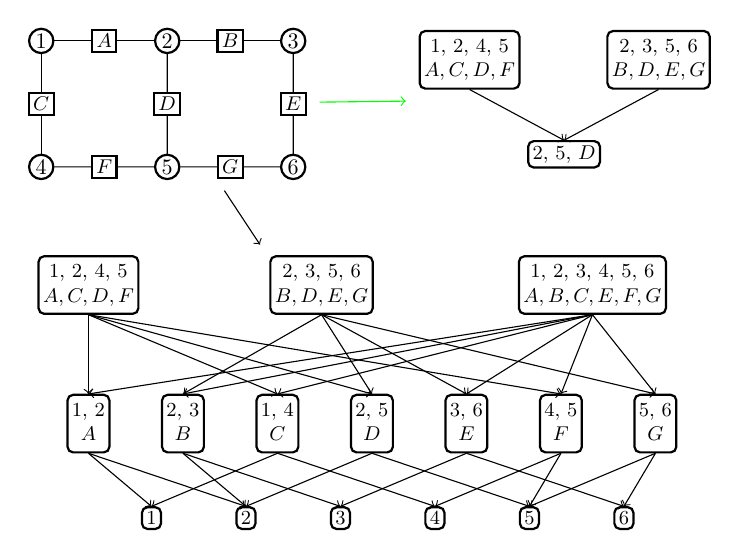
\begin{tikzpicture}
      \tikzstyle{cnode} = [thick, draw=black, circle, inner sep = 1pt,  align=center]
      \tikzstyle{nnode} = [thick, rectangle, rounded corners = 0pt,draw,inner sep = 2pt]

      %%%%%%%%%%%%%%%%%%%%%%%%%%%%%% 
      %% The 2-by-3 factor graph
      %%%%%%%%%%%%%%%%%%%%%%%%%%%%%% 
      \begin{scope}[scale=0.8, every node/.append style={transform shape}, local bounding box=grid]
        \node[cnode] (x1) at (0,0) {1};
        \node[cnode] (x2) at (2,0) {2};
        \node[cnode] (x3) at (4,0) {3};

        \node[cnode] (x4) at (0,-2) {4};
        \node[cnode] (x5) at (2,-2) {5};
        \node[cnode] (x6) at (4,-2) {6};

        \node[nnode] (fa) at (1,0) {\small$A$};
        \node[nnode] (fb) at (3,0) {\small$B$};

        \node[nnode] (fc) at (0,-1) {\small$C$};
        \node[nnode] (fd) at (2,-1) {\small$D$};
        \node[nnode] (fe) at (4,-1) {\small$E$};
        
        \node[nnode] (ff) at (1,-2) {\small$F$};
        \node[nnode] (fg) at (3,-2) {\small$G$};


        \draw[-] (x1) -- (fa);
        \draw[-] (x1) -- (fc);

        \draw[-] (x2) -- (fa);
        \draw[-] (x2) -- (fb);
        \draw[-] (x2) -- (fd);

        \draw[-] (x3) -- (fb);
        \draw[-] (x3) -- (fe);

        \draw[-] (x4) -- (fc);
        \draw[-] (x4) -- (ff);

        \draw[-] (x5) -- (fd);
        \draw[-] (x5) -- (ff);
        \draw[-] (x5) -- (fg);

        \draw[-] (x6) -- (fe);
        \draw[-] (x6) -- (fg);

      \end{scope}
      %%%%%%%%%%%%%%%%%%%%%%%%%%%%%% 
      %% The 2-layer region graph
      %%%%%%%%%%%%%%%%%%%%%%%%%%%%%% 
      \begin{scope}[scale=0.8, every node/.append style={transform shape}, xshift=6.8cm, yshift=-0.3cm, local bounding box=rg2]
        \tikzstyle{rnode} = [thick, rectangle, rounded corners = 2pt,minimum size = 0.0cm,draw,inner sep = 2pt]
        \node[rnode] (r01) at (0,0) {\small \begin{tabular}[x]{@{}c@{}}1, 2, 4, 5 \\ $A,C,D,F$ \end{tabular}};
        \node[rnode] (r02) at (3,0) {\small \begin{tabular}[x]{@{}c@{}}2, 3, 5, 6\\ $B,D,E,G$ \end{tabular}};
        \node[rnode] (r11) at (1.5, -1.5) {\small 2, 5, $D$};

        \draw[->] (r01.south) -- (r11.north);
        \draw[->] (r02.south) -- (r11.north);
      \end{scope}

      %%%%%%%%%%%%%%%%%%%%%%%%%%%%%% 
      %% The 3-layer region graph
      %%%%%%%%%%%%%%%%%%%%%%%%%%%%%% 
      \begin{scope}[xshift=0.6cm, yshift=-3.1cm,scale=0.8, every node/.append style={transform shape},local bounding box=rg3]
        \tikzstyle{rnode} = [thick, rectangle, rounded corners = 2pt,minimum size = 0.0cm,draw,inner sep = 2pt]
        \node[rnode] (r01) at (0,0) {\small\begin{tabular}[x]{@{}c@{}}1, 2, 4, 5 \\ $A,C,D,F$ \end{tabular}};
        \node[rnode] (r02) at (3.7,0) {\small\begin{tabular}[x]{@{}c@{}}2, 3, 5, 6\\ $B,D,E,G$ \end{tabular}};
        \node[rnode] (r03) at (8,0) {\small\begin{tabular}[x]{@{}c@{}}1, 2, 3, 4, 5, 6\\ $A,B,C,E,F,G$ \end{tabular}};
        \begin{scope}[yshift=-0.2cm]
          \node[rnode] (r11) at (0, -2.0) {\small\begin{tabular}[x]{@{}c@{}}1, 2\\ $A$ \end{tabular}};
          \node[rnode] (r12) at (1.5, -2.0) {\small\begin{tabular}[x]{@{}c@{}}2, 3\\ $B$ \end{tabular}};
          \node[rnode] (r13) at (3, -2.0) {\small\begin{tabular}[x]{@{}c@{}}1, 4\\ $C$ \end{tabular}};
          \node[rnode] (r14) at (4.5, -2.0) {\small\begin{tabular}[x]{@{}c@{}}2, 5\\ $D$ \end{tabular}};
          \node[rnode] (r15) at (6, -2.0) {\small\begin{tabular}[x]{@{}c@{}}3, 6\\ $E$ \end{tabular}};
          \node[rnode] (r16) at (7.5, -2.0) {\small\begin{tabular}[x]{@{}c@{}}4, 5\\ $F$ \end{tabular}};
          \node[rnode] (r17) at (9, -2.0) {\small\begin{tabular}[x]{@{}c@{}}5, 6\\ $G$ \end{tabular}};

          \begin{scope}[yshift=0.5cm]
            \node[rnode] (r21) at (1, -4) {\small 1};
            \node[rnode] (r22) at (2.5, -4) {\small 2};
            \node[rnode] (r23) at (4, -4) {\small 3};
            \node[rnode] (r24) at (5.5, -4) {\small 4};
            \node[rnode] (r25) at (7, -4) {\small 5};
            \node[rnode] (r26) at (8.5, -4) {\small 6};
          \end{scope}
        \end{scope}
        % edge level0 to level1
        \draw[->] (r01.south) -- (r11.north);
        \draw[->] (r03.south) -- (r11.north);

        \draw[->] (r02.south) -- (r12.north);
        \draw[->] (r03.south) -- (r12.north);

        \draw[->] (r01.south) -- (r13.north);
        \draw[->] (r03.south) -- (r13.north);

        \draw[->] (r01.south) -- (r14.north);
        \draw[->] (r02.south) -- (r14.north);

        \draw[->] (r02.south) -- (r15.north);
        \draw[->] (r03.south) -- (r15.north);

        \draw[->] (r01.south) -- (r16.north);
        \draw[->] (r03.south) -- (r16.north);

        \draw[->] (r02.south) -- (r17.north);
        \draw[->] (r03.south) -- (r17.north);

        % edge level1 to level2
        \draw[->] (r11.south) -- (r21.north);
        \draw[->] (r13.south) -- (r21.north);

        \draw[->] (r11.south) -- (r22.north);
        \draw[->] (r12.south) -- (r22.north);
        \draw[->] (r14.south) -- (r22.north);


        \draw[->] (r12.south) -- (r23.north);
        \draw[->] (r15.south) -- (r23.north);

        \draw[->] (r13.south) -- (r24.north);
        \draw[->] (r16.south) -- (r24.north);

        \draw[->] (r14.south) -- (r25.north);
        \draw[->] (r16.south) -- (r25.north);
        \draw[->] (r17.south) -- (r25.north);

        \draw[->] (r15.south) -- (r26.north);
        \draw[->] (r17.south) -- (r26.north);
      \end{scope}
      \draw[green, ->, shorten >=5pt, shorten <=5pt] (grid) -- (rg2);
      \draw[->, shorten >=5pt, shorten <=5pt] (grid) -- (rg3);
      

    \end{tikzpicture}
    \column{0.3\textwidth}
    \begin{itemize}[label=\textbullet]
    \item Clustering nodes
    \item level/layer-wise
    \item Hierarchical
    \item Msg. Scheduling
    \item ...
    \item See Section 4.1
      
    \end{itemize}
  \end{columns}

  
\end{frame}
\begin{frame}{RENN: Region-based Energy Neural Network}
  The \textbf{region-based free energy} of a region graph is
  \begin{equation*}
    F_R(\Bb; \bm{\theta}) = \sum_{R\in \Rr} \underbrace{c_R}_{\text{Counting number}} \sum_{\bm{x}_R}\underbrace{b_R(\bm{x}_R)}_{\text{Belief on region R}} (\underbrace{E_R(\bm{x}_R; \bm{\theta}_R)}_{\text{Region average energy}} + \ln{b_R}(\bm{x}_R)),
  \end{equation*}
  \begin{itemize}[label=$\bullet$]
  \item counting number: balance the contribution of each region
  \item region average energy: $- \sum_{a\in A_R} \ln{\phi_a(\bm{x}_a; \bm{\theta}_a)}$
  \end{itemize}
  
  \only<2>{
  
  \begin{columns}
    \column{0.3\textwidth}
    \centering
    \begin{tikzpicture}
      
      \tikzstyle{cnode} = [thick, draw=black, circle, inner sep = 1pt,  align=center]
      \tikzstyle{nnode} = [thick, rectangle, rounded corners = 0pt,draw,inner sep = 2pt]
      
      \begin{scope}[xshift=0cm, scale=0.6, every node/.append style={transform shape}, local bounding box=rg2]
        \tikzstyle{rnode} = [thick, rectangle, rounded corners = 2pt,minimum size = 0.0cm,draw,inner sep = 2pt]
        \node[rnode] (r01) at (0,0) {\small \begin{tabular}[x]{@{}c@{}}1, 2, 4, 5 \\ $A,C,D,F$ \end{tabular}};
        \node[rnode] (r02) at (3,0) {\small \begin{tabular}[x]{@{}c@{}}2, 3, 5, 6\\ $B,D,E,G$ \end{tabular}};
        \node[rnode] (r11) at (1.5, -2.1) {\small 2, 5, $D$};

        \draw[->] (r01.south) -- (r11.north);
        \draw[->] (r02.south) -- (r11.north);

      \end{scope}
      \begin{scope}
        \begin{scope}[yshift=-2cm, scale=0.6, every node/.append style={transform shape}]
          \tikzstyle{cnode} = [thick, draw=black, circle, inner sep = 1pt,  align=center]
          
          \tikzstyle{rnode} = [thick, circle, rounded corners = 2pt,minimum size = 0.0cm,draw,inner sep = 0.5pt]
          \node[rnode] (r01) at (0,0) {$R_1^{[0]}$};
          \node[rnode] (r02) at (3,0) {$R_2^{[0]}$};
          \node[rnode] (r11) at (1.5, -2.1) {$R_1^{[1]}$};
        \end{scope}
        \tikzstyle{nnode} = [dashed, draw=blue, rectangle, rounded corners = 2pt, inner sep = 4pt]
        \node[nnode, fit=(r01)(r02), label=right:{$\Rr_0$,root}] {};
        \node[nnode, fit=(r11), label=right:$\Rr_1$] {};

        \draw[->] (r01.south) -- (r11.north);
        \draw[->] (r02.south) -- (r11.north);
      \end{scope}
    \end{tikzpicture}
    
    \column{0.7\textwidth}
    \centering
    \begin{tikzpicture}
      \tikzstyle{enode} = [thick, draw=black, ellipse, inner sep = 2pt,  align=center]
      \tikzstyle{cnode} = [thick, draw=black, circle, inner sep = 0.0pt,  align=center]
      \tikzstyle{nnode} = [thick, rectangle, rounded corners = 0pt,draw,inner sep = 2pt]
      \begin{scope}[xshift=-1cm, yshift=-1.3cm, scale=0.6]
        \node[enode, rotate=90] (em) at (-2.5,0) {Embedings};
        \node[enode, rotate=90] (nn) {Neural Network};
      \end{scope}
      
      % level0 regions
      \begin{scope}[scale=0.6]
        \node[cnode] (r01) at (1, 0) {\tiny$R_1^{[0]}$};
        \node[cnode] (r02) at (1, -1) {\tiny$R_2^{[0]}$};
        \node[cnode] (r03) at (1, -2) {\tiny$R_3^{[0]}$};
        \node[cnode] (r04) at (1, -3) {\tiny$R_4^{[0]}$};
        \node[cnode] (r05) at (1, -4) {\tiny$R_5^{[0]}$};
        \node[label=below:$\Rr_0$, draw,rounded corners = 2pt, inner sep=1mm, fit=(r01) (r05)] {};
      \end{scope}

      \draw[->] (nn.351.9) |- (r01);
      \draw[->] (nn.340) |- (r02);
      \draw[->] (nn.295) |- (r03);
      \draw[->] (nn.210) |- (r04);
      \draw[->] (nn.191) |- (r05);

      \draw[->] (em) -- (nn);


      % level 1 regions
      \begin{scope}[xshift=1.5cm, yshift=-0.2cm, scale=0.6]
        \node[cnode] (r11) at (1, 0) {\tiny$R_1^{[1]}$};
        \node[cnode] (r12) at (1, -1) {\tiny$R_2^{[1]}$};
        \node[cnode] (r13) at (1, -2) {\tiny$R_3^{[1]}$};
        \node[cnode] (r14) at (1, -3) {\tiny$R_4^{[1]}$};
        \node[label=below:$\Rr_1$, draw, rounded corners = 2pt, inner sep=1mm, fit=(r11) (r14)] {};
      \end{scope}

      
      
      % level 1 regions
      \begin{scope}[xshift=3cm, yshift=-0.2cm, scale=0.6]
        \node[cnode] (r21) at (1, 0) {\tiny$R_1^{[2]}$};
        \node[cnode] (r22) at (1, -1) {\tiny$R_2^{[2]}$};
        \node[cnode] (r23) at (1, -2) {\tiny$R_3^{[2]}$};
        \node[cnode] (r24) at (1, -3) {\tiny$R_4^{[2]}$};
        \node[label=below:$\Rr_2$, draw, rounded corners = 2pt, inner sep=1mm, fit=(r21) (r24)] {};
      \end{scope}

      \draw[->] (r01) -- (r11);
      \draw[->] (r03) -- (r11);

      \draw[->] (r02) -- (r12);
      \draw[->] (r04) -- (r12);
      \draw[->] (r05) -- (r12);

      \draw[->] (r01) -- (r13);
      \draw[->] (r04) -- (r13);

      \draw[->] (r03) -- (r14);
      \draw[->] (r05) -- (r14);


      \draw[->] (r11) -- (r21);
      \draw[->] (r14) -- (r21);

      \draw[->] (r11) -- (r22);
      \draw[->] (r13) -- (r22);

      \draw[->] (r12) -- (r23);
      \draw[->] (r14) -- (r23);

      \draw[->] (r12) -- (r24);
      \draw[->] (r13) -- (r24);

      \draw[green, ->] (-2.5,0.5) --node[black,midway,above]{Amortize root beliefs} (0.5,0.5);
      \draw[green, ->] (1,0.5) --node[text width=2.8cm, black,midway,above]{Accumulate belief consistency error} (3.5,0.5);
      \draw[green, ->] (3.5,-3.2) --node[text width=2.8cm, black,midway,below]{Back-propagation} (-2.5,-3.2);
      
      
    \end{tikzpicture}
  \end{columns}
  }
\end{frame}

\begin{frame}{RENN}
  \onslide<1->{
    Non-root belief: \\
    \begin{center}
    \begin{tikzpicture}
        \begin{scope}[yshift=-2cm, scale=0.6, every node/.append style={transform shape}]
          \tikzstyle{cnode} = [thick, draw=black, circle, inner sep = 1pt,  align=center]
              \tikzstyle{rnode} = [thick, circle, rounded corners = 2pt,minimum size = 0.0cm,draw,inner sep = 0.5pt]
          \node[rnode] (r01) at (0,0) {$R_1^{[0]}$};
          \node[rnode] (r02) at (3,0) {$R_2^{[0]}$};
          \node[rnode] (r11) at (1.5, -2.1) {$R_1^{[1]}$};
        \end{scope}

        \draw[->] (r01.south) -- node[align=center, text width=3cm, black,midway,left]{\tiny Marginalize to child region} (r11.north);
        \draw[->] (r02.south) -- node[align=center, text width=3cm, black,midway,right]{\tiny Marginalize to child region}(r11.north);
        \node[below=0.1cm of r11] {\tiny Average incoming marginalization from parents};
      \end{tikzpicture}
    \end{center}
    \vskip -0.5cm
    Objective of RENN:\\
    \begin{equation*}
      \min_{\text{\begin{tabular}{c}parameter \\of NN\end{tabular}}} \mathrm{\underbrace{\textbf{region-based free energy} (F_R)}_{\text{Assumulated average of all regions}}} + \underbrace{\mathrm{\textbf{panelty on belief consistency} }}_{\text{Recursively computed via levels of region graph}}
    \end{equation*}
  }
  \\
  \only<2->{
    RENN Inference:
    \begin{center}
    \begin{tikzpicture}
      %%%%%%%%%%%%%%%%%%%%%%%%%%%%%%%%%%%%%%%%%%%%%%%%%% 
      %% use of RENN
      %%%%%%%%%%%%%%%%%%%%%%%%%%%%%%%%%%%%%%%%%%%%%%%%%% 
      \tikzstyle{cnode} = [thick, draw=blue, rounded corners = 4pt, rectangle, inner sep = 4pt,  align=center]
      \tikzstyle{nnode} = [thick, rectangle, rounded corners = 0pt,draw,inner sep = 2pt]
      \tikzstyle{rnode} = [thick, rectangle, rounded corners = 2pt,minimum size = 0.0cm,draw,inner sep = 4pt]
      \begin{scope}[scale=0.8, every node/.append style={transform shape} ]
        \node[rnode] (r01) at (-1,0) {MRF};
        \node[rnode, right=of r01] (r02) {\begin{tabular}[x]{@{}c@{}} Construct Region Graph\\ {\tiny Tree-robust conditon} \\ {\tiny $+$ Cluster Variation Method} \\ {\tiny $+$ Validity} \\ {\tiny Section 4.3.2}\end{tabular}};
        \node[rnode, right=of r02] (r03) {\begin{tabular}{c}Free Energy Optimization\\ {\tiny Backpropagation}\\ {\tiny Gradient descent} \\ Consistency Regularization\\ {\tiny Direct root belief reps.} \\ {\tiny Recursive non-root belief compt.}\end{tabular}};
        \node[rnode, right=of r03] (r04) {\begin{tabular}{c}Read out: \\Beliefs or \\Partition\end{tabular}};
      \end{scope}
      \begin{scope}[on background layer]
        \node[cnode, fit=(r02)(r03), label=below:{RENN}, draw=black, fill=blue, opacity=0.2] (renn) {};
      \end{scope}
      \draw[->] (r01) -- (renn);
      \draw[->] (renn) -- (r04);
      \draw[->] (r02) -- (r03);
    \end{tikzpicture}
    \end{center}
  }
  % \onslide<2->{
  %   Learning alternatives of MRFs
  %   \begin{columns}
  %     \column{0.5\textwidth}
  %     learn with customized optm.
  %     \begin{align*}
  %       \pd{\log{p}(\bm{x};\bm{\theta})}{\bm{\theta}_a} = &\pd{\log{{\phi_a}(\bm{x}_a; \bm{\theta}_a)}}{\bm{\theta}_a} \\
  %                                                         &- \underbrace{\EE_{p(\bm{x}_a; \bm{\theta})}\left[ \pd{\log{{\phi_a}(\bm{x}_a; \bm{\theta}_a)}}{\bm{\theta}_a} \right]}_{\text{est. by beliefs}}.
  %     \end{align*}
  %     \column{0.5\textwidth}
  %     learn with auto-grads
  %     \begin{align*}
  %       \max_{\bm{\theta}} \log{p(\bm{x}; \bm{\theta})} =  &\max_{\bm{\theta}}\sum_{a}\log{ \psi_a(\bm{x}_a; \bm{\theta}_a) } \\
  %                                                          &\underbrace{ -\log{Z(\bm{\theta})}}_{\text{\begin{tabular}{c}ets. by the\\ Helmholtz free energy\\ $-\log{Z(\bm{\theta})} \simeq F_R$ \end{tabular}}}.
  %     \end{align*}
  %   \end{columns}
  % }
\end{frame}
\begin{frame}{Insights of RENN}
  \begin{block}{Generalization}
    Bethe free energy can be recovered from region-based free energy:
    \begin{itemize}[label=\textbullet]
    \item two-level region graph representation
    \item constraint that each region can contain at most one factor node
    \end{itemize}
    {\tiny Section 4.2.1}
  \end{block}
  \begin{block}{Attributes of RENN}
    \begin{itemize}[label=\textbullet]
    \item RENN requires neither sampling technique nor training data (ground-truth marginal probabilities) in performing inference tasks;
    \item RENN does gradient descent w.r.t. its neural network parameter instead of iterative message-passing, and returns approximation of marginal probabilities and partition estimation in one-shot
    \item No message propagation, thus no need of message scheduling
    \item Competitive performance and efficiency
    \end{itemize}
  \end{block}
\end{frame}

\begin{frame}{Some Numerical Comparisons}
  
  Ising model: $p(\bm{x}; \bm{\theta}) = \frac{1}{Z(\bm{\theta})}\exp{(\sum_{(i,j)\in \Ee_F} J_{ij} x_i x_j + \sum_{i\in \Vv}h_i x_i)}$, $\bm{x} \in \{-1, 1\}^{N}$,
  \begin{itemize}[label=$\bullet$]
  \item $J_{ij}$ is the pairwise log-potential between node $i$ and $j$, $J_{ij}\sim \Nn(0,1)$
  \item  $h_i$ is the node log-potential for node $i$, $h_i \sim \Nn(0, \gamma^{2})$
  \end{itemize}
  
  Inference on grid graph ($\gamma=0.1$). 
  \begin{adjustbox}{width=1\textwidth}
    \begin{tabular}{lcccccccc}
      \toprule
      Metric & $n$ & Mean Field & Loopy BP & Damped BP & GBP & Inference Net & RENN \\
      \midrule
      \multirow{4}{*}{\begin{tabular}[x]{@{}c@{}}$\ell_1$\\error \end{tabular} }
             &    25   &$0.271 \pm 0.051$ &  $0.086 \pm 0.078$ & $0.084 \pm 0.076$ & $0.057 \pm 0.024$ & $0.111 \pm 0.072$ & \textbf{0.049} $\pm$ 0.078 \\

             &    100   & $0.283 \pm 0.024$ &  $0.085 \pm 0.041$ & $0.062 \pm 0.024$ & $0.064 \pm 0.019$ & $0.074 \pm 0.034$ & \textbf{0.025} $\pm$ 0.011 \\

             &    225   & $0.284 \pm 0.019$ &  $0.100 \pm 0.025$ & $0.076 \pm 0.025$ & $0.073 \pm 0.013$ & $ 0.073 \pm 0.012$ & \textbf{0.046} $\pm$ 0.011 \\

             &    400   & $0.279 \pm 0.014$ &  $0.110 \pm 0.016$ & $0.090 \pm 0.016$ & $0.079 \pm 0.009$ & $ 0.083 \pm 0.009$ & \textbf{0.061} $\pm$ 0.009 \\

      \midrule
      \multirow{4}{*}{\begin{tabular}[x]{@{}c@{}}Corre-\\lation\\ $\rho$ \end{tabular}}
             &   25    & 0.633 $\pm$ 0.197  &  0.903 $\pm$ 0.114  &  0.905 $\pm$ 0.113  &  0.923 $\pm$ 0.045  &  0.866$\pm$ 0.117 &  \textbf{0.951} $\pm$ 0.112 \\

             &   100   & 0.582 $\pm$ 0.112  &  0.827 $\pm$ 0.134  &  0.902 $\pm$ 0.059  &  0.899 $\pm$ 0.043  &  0.903$\pm$ 0.049 &   \textbf{0.983} $\pm$ 0.012 \\

             &   225   & 0.580 $\pm$ 0.080  &  0.801 $\pm$ 0.078  &  0.863 $\pm$ 0.088  &  0.869 $\pm$ 0.037  & 0.873 $\pm$ 0.037 &  \textbf{0.949} $\pm$ 0.022 \\

             &   400   & 0.596 $\pm$ 0.054  &  0.779 $\pm$ 0.059  &  0.822 $\pm$ 0.047  &  0.852 $\pm$ 0.024  & 0.841 $\pm$ 0.028 &  \textbf{0.912} $\pm$ 0.025 \\

      \midrule
      \multirow{4}{*}{\begin{tabular}[x]{@{}c@{}}$\log{Z}$ \\error\end{tabular}}
             &   25    & 2.512 $\pm$ 1.060  &  0.549 $\pm$ 0.373  &  0.557 $\pm$ 0.369  &  \textbf{0.169} $\pm$ 0.142  &  0.762 $\pm$ 0.439  &  0.240 $\pm$ 0.140 \\

             &  100    & 13.09 $\pm$ 2.156  &  1.650 $\pm$ 1.414  &  1.457 $\pm$  1.365 &  \textbf{0.524} $\pm$ 0.313  &  2.836 $\pm$ 2.158  & 1.899 $\pm$ 0.495 \\

             &  225    & 29.93 $\pm$ 4.679  &  3.348 $\pm$ 1.954  &  3.423 $\pm$ 2.157  &  \textbf{1.008} $\pm$ 0.653  &  3.249 $\pm$ 2.058  & 4.344 $\pm$ 0.813  \\

             &  400    & 51.81 $\pm$ 4.706  &  5.738 $\pm$ 2.107  &  5.873$\pm$ 2.211   &  \textbf{1.750} $\pm$ 0.869  &  3.953 $\pm$ 2.558  & 7.598 $\pm$ 1.146 \\

      \bottomrule
    \end{tabular}
  \end{adjustbox}
  \begin{itemize}[label=$\bullet$]
  \item $\ell_1$ error of beliefs v.s. true
  \item correlation $\rho$ between true and approximate marginals,
  \item $\log{Z}$ error, true v.s. free energy approximation.
  \end{itemize}
  
\end{frame}
\begin{frame}
  {Some Numerical Comparisons}
  {Richer Comparisons}
  Inference on grid and complete graphs.
  \begin{table}
    \vskip -0.1in
    \begin{adjustbox}{width=1\textwidth}
      \begin{small}
        \begin{tabular}{cl c ccccccc}
          \toprule
          {}&{}& Metric & {} & Mean Field & Loopy BP & Damped BP & GBP & Inference Net & RENN \\
          \midrule
          \multirow{4}{*}{\rotatebox[origin=c]{90}{\begin{tabular}{c}High Temp\\-erature\end{tabular}}}%  &
            &\multirow{4}{*}{\rotatebox[origin=c]{0}{\begin{tabular} [x]{@{}c@{}} Complete graph \\ N=16 \\$J_{ij}\sim \Nn(0,1)$ \\ $h_i \sim \Nn(0, \gamma^{2})$ \end{tabular}}} &
                                                                                                                                                                                    \multirow{2}{*}{\begin{tabular}[x]{@{}c@{}}$\ell_1$-\\error\end{tabular}}
            & $\gamma=1$   &  0.273 $\pm$ 0.086  &  0.239 $\pm$ 0.059  &  0.239 $\pm$ 0.059  &  0.260 $\pm$ 0.086  &  0.249 $\pm$ 0.067  &  \textbf{0.181} $\pm$ 0.092  \\
            & &       &  $\gamma=4$    &  0.197 $\pm$0.049   &  0.181 $\pm$ 0.035  &  0.180 $\pm$ 0.034  &  0.210 $\pm$ 0.070  &  0.174 $\pm$ 0.030  &  \textbf{0.125} $\pm$ 0.050  \\
          \cmidrule{3-10}
            &&\multirow{2}{*}{\begin{tabular}[x]{@{}c@{}}$\log{Z}$ \\error\end{tabular}}
            &  $\gamma=1$    &  20.66 $\pm$ 5.451  &  178.7 $\pm$ 22.18  &  178.9 $\pm$ 21.88  &  153.3 $\pm$ 25.29  &  213.6 $\pm$ 12.75  &  \textbf{14.41} $\pm$ 4.135  \\
            &&      &  $\gamma=4$    &  \textbf{10.74} $\pm$ 7.385  &  565.7 $\pm$ 73.33  &  566.1 $\pm$ 73.13  &  106.0 $\pm$ 54.43  &  588.3 $\pm$ 62.58  &  14.72 $\pm$ 4.155  \\
          
          
          \bottomrule
          {\multirow{4}{*}{\rotatebox[origin=c]{90}{\begin{tabular}{c}Low Temp\\-erature\end{tabular}}}}&\multirow{4}{*}{\rotatebox[origin=c]{0}{\begin{tabular} [x]{@{}c@{}} Grid graph \\ N=100\\ $J_{ij}\sim \Uu(-u,u)$ \\ $h_i \sim \Uu(-1, 1)$ \end{tabular}}}
            &\multirow{2}{*}{\begin{tabular}[x]{@{}c@{}}$\ell_1$\\error \end{tabular} }
            &    5   & $0.257 \pm 0.065$ &  $0.115 \pm 0.071$ & $0.120 \pm 0.073$ & $0.250 \pm 0.024$ & $ 0.164 \pm 0.036$ & \textbf{0.100} $\pm$ 0.046 \\

            &&&    15  & $0.328 \pm 0.068$ &  $0.228 \pm 0.088$ & $0.267 \pm 0.147$ & $0.303 \pm 0.026$ & $ 0.279 \pm 0.024$ & \textbf{0.207} $\pm$ 0.054 \\
          \cmidrule{3-10}
            & &\multirow{2}{*}{\begin{tabular}[x]{@{}c@{}}$\log{Z}$ \\error\end{tabular}}
            &  5     & 42.65 $\pm$ 17.86  &  7.346 $\pm$ 7.744  &  \textbf{5.444} $\pm$ 4.811  &  {8.369} $\pm$ 7.401  &  65.60 $\pm$ 8.786  & 11.34 $\pm$ 4.724 \\
            &&      &  15    & 164.9 $\pm$ 56.07  &  58.40 $\pm$ 41.36  &  101.9 $\pm$ 54.31  &  \textbf{23.10} $\pm$ 15.06  &  224.3 $\pm$ 25.52  & 78.85 $\pm$ 15.08 \\
          \bottomrule
        \end{tabular}
      \end{small}
    \end{adjustbox}
    \vskip -0.1in
  \end{table}
  {Average consumed time per inference instance (unit: second)}
  \begin{table}
    
    \vskip -0.1in
    \centering
    \begin{adjustbox}{width=0.98\textwidth}
      \begin{tabular}{lcccccc}
        \toprule
        {} &  Mean Field & Loopy BP & Damped BP & GBP & Inference Net & RENN \\
        \toprule
        Grid $\Gg$, $N=400$, $J_{ij}\sim \Nn(0,1), h_i\sim\Nn(0,0.1^2)$ & 9.897 & 425.0 & 328.3 & 286.3 & 74.41 & 101.0 \\
        Complete $\Gg$, $N=16$, $J_{ij}\sim \Nn(0,1), h_i\sim\Nn(0,1)$ & 0.457 & 0.777 & 1.285 & 14.29 &  12.45  & 16.16\\
        Grid $\Gg$, $N=100$, $J_{ij}\sim \Uu(-15,15), h_i\sim\Uu(-1,1)$ & 2.314 & 253.3 & 229.3 & 53.72 & 103.4 & 79.38 \\
        Complete $\Gg$, $N=9$, $J_{ij}\sim \Uu(-15,15), h_i\sim\Uu(-1,1)$ & 0.502 & 15.86 & 18.23 & 3.213 & 17.21 & 7.857 \\
        \bottomrule
      \end{tabular}
    \end{adjustbox}
  \end{table}
\end{frame}
%%% Local Variables:
%%% mode: latex
%%% TeX-master: "../ppgm_slide"
%%% End:
